\documentclass[a4paper,12pt]{article}
\usepackage[utf8]{inputenc}
\usepackage{amsmath}
\usepackage{graphicx}
\usepackage{listings}
\usepackage{caption}
\usepackage{float}
\usepackage{tikz}
\usepackage{pgfplots}
\pgfplotsset{compat=1.18}
\usepackage{longtable}
\usepackage{pgfplots}
\usepackage{xcolor}
\lstdefinestyle{mystyle}{
    keywordstyle=\color{blue},       % kolor słów kluczowych
    numberstyle=\tiny\color{gray},   % kolor numerów linii
    basicstyle=\ttfamily\footnotesize, % styl podstawowy
    breaklines=true,                 % łamanie długich wierszy
    captionpos=b,                    % pozycja podpisu
    numbers=left,                    % numery linii po lewej stronie
    numbersep=1pt,                   % odstęp numerów linii
    showspaces=false,                % nie pokazuj spacji
    tabsize=2                        % rozmiar tabulacji
}

\lstset{style=mystyle}

\title{Analiza Algorytmów Sortowania}
\author{Ksawery Józefowski\\Politechnika Wrocławska}
\date{\today}

\begin{document}

\maketitle

\tableofcontents
\newpage

\section{Wstęp}
W ramach Listy 2 zaimplementowano i przeanalizowano 4 algorytmy sortowania: \textit{Insertion Sort}, \textit{Bucket Sort}, \textit{Quick Sort} oraz \textit{Radix Sort}. Każdy z algorytmów został zmodyfikowany: \textit{Quick Sort} dzieli tablice na 3 części, \textit{Bucket Sort} działa nie tylko na przedziale [0-1], \textit{Radix Sort} sortuje również liczby ujemne, a \textit{Insertion Sort} działa na listach. Celem projektu jest porównanie \textit{Bucket Sorta} z \textit{Quick Sortem} jak i również porównanie \textit{Radix Sorta} dla różnych podstaw.

\section{Fragmenty Kodów}
Poniżej przedstawiono najciekawsze fragmenty kodu dla wybranych algorytmów.

\subsection{Radix Sort}
Algorytm \textit{Radix Sort} to nieporównawczy algorytm sortujący, który działa poprzez sortowanie liczb na podstawie ich cyfr. Wykorzystuje on stabilny algorytm sortujący, taki jak \textit{Counting Sort}, do sortowania elementów na podstawie poszczególnych cyfr. Proces sortowania w \textit{Radix Sort} jest iteracyjny i przebiega od najmniej znaczącej cyfry do najbardziej znaczącej.

\begin{itemize}
    \item Algorytm najpierw identyfikuje największą liczbę w tablicy, co pozwala określić liczbę iteracji wymaganych do posortowania na podstawie najbardziej znaczącej cyfry.
    \item Następnie wykonuje \textit{Counting Sort} dla każdej cyfry, zaczynając od 
    najmniej znaczącej. 
    \item W każdej iteracji elementy są sortowane w oparciu o jedną cyfrę, przy zachowaniu stabilności algorytmu, co pozwala zachować poprawną kolejność elementów między iteracjami.
\end{itemize}

Dzięki tej metodzie, \textit{Radix Sort} jest w stanie sortować liczby całkowite w czasie \(O(b \cdot (n + d))\), gdzie:
\begin{itemize}
    \item \(n\) to liczba elementów w tablicy,
    \item \(b\) to liczba cyfr w największej liczbie,
    \item \(d\) to podstawa systemu liczbowego (np. 10 dla systemu dziesiętnego).
\end{itemize}

\subsection{Radix Sort Negative}
Algorytm \textit{Radix Sort Negative} jest modyfikacją klasycznego algorytmu \textit{Radix Sort}, która została zaprojektowana z myślą o sortowaniu liczb zarówno dodatnich, jak i ujemnych. Zmiana polega na rozszerzeniu zakresu zliczania, aby mogły być obsługiwane liczby ujemne.

\begin{itemize}
    \item Zamiast tylko zliczać cyfry liczb dodatnich, algorytm rozszerza zakres zliczania, aby uwzględnić zarówno liczby dodatnie, jak i ujemne.
    \item Proces sortowania dla liczb ujemnych wymaga przesunięcia cyfr, aby odpowiednio obsłużyć te liczby.
    \item Algorytm wykonuje iteracyjne sortowanie przez cyfry, podobnie jak w przypadku klasycznego \textit{Radix Sort}, ale z uwzględnieniem liczb ujemnych.
\end{itemize}

Dzięki tej modyfikacji, \textit{Radix Sort Negative} jest w stanie poprawnie sortować liczby całkowite, niezależnie od ich znaku, w czasie podobnym do \textit{Radix Sort}, tj. \(O(d \cdot (n + b))\). Jest to efektywny sposób sortowania liczb zarówno dodatnich, jak i ujemnych, przy zachowaniu stabilności algorytmu.

Wersja \textit{Radix Sort Negative} może być użyteczna w przypadkach, gdy musimy posortować zbiory danych zawierające zarówno liczby dodatnie, jak i ujemne, bez konieczności oddzielnego przetwarzania obu typów liczb.


\newpage
\begin{lstlisting}[language=C++,caption=Radix z obsługą ujemnych liczb]
void radixSort_negative(int arr[], int n, int base, unsigned long long& comparisons, unsigned long long& assignments) {
    const int size = base * 2 - 1;
    auto output = new int[n];

    for (int pos = 1; ; pos *= base) {
        int counter[size]{};

        bool done = true;
        for (int i = 0; i < n; i++) {
            int d = arr[i] / pos;
            assignments++;
            ++counter[d % base + size / 2];
            done &= (d == 0);
        }
        if (done)
            break;

        for (int i = 1; i < size; i++)
            counter[i] += counter[i - 1];

        for (int i = n; i-- > 0; ) {
            output[--counter[arr[i] / pos % base + size / 2]] = arr[i];
            assignments++;
        }

        for (int i = 0; i < n; i++) {
            arr[i] = output[i];
            assignments++;
        }
    }

    delete[] output;
}

\end{lstlisting}
\newpage

\subsection{Bucket Sort}
Algorytm \textit{Bucket Sort} jest algorytmem sortującym opartym na rozdzieleniu elementów na różne "wiadra" (ang. *buckets*), a następnie posortowaniu ich wewnętrznie, zazwyczaj za pomocą algorytmu \textit{Insertion Sort}. Każde wiadro zawiera elementy, które są "bliskie" siebie w kontekście ich wartości.

\begin{itemize}
    \item Na początku algorytm znajduje najmniejszą i największą wartość w zbiorze, co pozwala na określenie zakresu wartości.
    \item Z zakresu tego obliczany jest rozmiar jednego wiadra, który jest równy różnicy między największą a najmniejszą wartością podzieloną przez liczbę elementów.
    \item Następnie każdy element jest przypisany do odpowiedniego wiadra na podstawie jego wartości.
    \item Każde wiadro jest następnie sortowane indywidualnie, a wynikowe posortowane elementy są łączone w jeden posortowany zbiór.
\end{itemize}

Algorytm \textit{Bucket Sort} może działać w czasie \(O(n + k)\), gdzie \(n\) to liczba elementów, a \(k\) to liczba wiader, jednakże jego wydajność zależy od jakości rozdzielenia elementów na wiadra oraz od zastosowanego algorytmu wewnętrznego do sortowania w wiadrach.

\subsection{Bucket Sort Mod}
\textit{Bucket Sort Mod} jest zmodyfikowaną wersją klasycznego algorytmu \textit{Bucket Sort}, która obsługuje przypadki, w których elementy nie mieszczą się w standardowym zakresie \(0\)-\(1\).

\begin{itemize}
    \item Algorytm zaczyna od obliczenia minimalnej i maksymalnej wartości w zbiorze danych, jak w klasycznym \textit{Bucket Sort}.
    \item Na podstawie tej informacji obliczany jest zakres wartości, a następnie liczba wiader, do których będą przypisane elementy. W tym przypadku zakres może być znacznie szerszy.
    \item Kluczową modyfikacją w tej wersji algorytmu jest możliwość pracy z liczbami spoza przedziału \(0\)-\(1\), co oznacza, że elementy są odpowiednio mapowane na wiadra w oparciu o ich wartość unormalizowane do zakresu 0-1.
    \item Każdy element jest przypisany do odpowiedniego wiadra, a następnie wiadra są sortowane, np. za pomocą \textit{Insertion Sort}. Po posortowaniu, elementy są scalane w jedno posortowane zestawienie.
\end{itemize}

Modyfikacja ta pozwala na sortowanie liczb z dowolnego zakresu, nie ograniczając się do przedziału \(0\)-\(1\). Złożoność czasowa algorytmu jest podobna do klasycznej wersji i wynosi \(O(n + k)\), gdzie \(n\) to liczba elementów, a \(k\) to liczba wiader. Poprawiona wersja jest bardziej elastyczna i może być używana do sortowania liczb o dowolnym zakresie wartości.

\begin{lstlisting}[language=C++,caption=Bucket sort z obsługą liczb spoza zakresu 0-1]
void bucketSort_Mod(double arr[], int n) {
    if (n <= 0) return;

    double minVal = arr[0], maxVal = arr[0];
    for (int i = 1; i < n; i++) {
        if (arr[i] < minVal) minVal = arr[i];
        if (arr[i] > maxVal) maxVal = arr[i];
    }

    int numBuckets = n;
    double bucketRange = (maxVal - minVal);

    Node** buckets = new Node*[numBuckets]();

    for (int i = 0; i < n; i++) {
        int bucketIndex = (arr[i] - minVal) / (maxVal - minVal) * n;
        if (bucketIndex == numBuckets) bucketIndex--;
        insert(buckets[bucketIndex], arr[i]);
    }

    for (int i = 0; i < numBuckets; i++) {
        insertionSort(buckets[i]);
    }

    int index = 0;
    for (int i = 0; i < numBuckets; i++) {
        Node* current = buckets[i];
        while (current != nullptr) {
            arr[index++] = current->data;
            Node* temp = current;
            current = current->next;
            delete temp;
        }
    }
    delete[] buckets;
}
\end{lstlisting}
\newpage
\subsection{QuickSort}
Algorytm \textit{QuickSort} jest algorytmem sortującym działającym na zasadzie "dziel i zwyciężaj" (ang. *divide and conquer*). Polega na wybieraniu elementu z tablicy jako tzw. "pivot" (punkt odniesienia), a następnie przekształca tablicę tak, aby wszystkie elementy mniejsze od pivota znajdowały się po jednej stronie, a większe po drugiej. Następnie algorytm rekurencyjnie sortuje obie części.

\begin{itemize}
    \item Na początku wybierany jest element pivot (zwykle ostatni element tablicy).
    \item Następnie wykonywana jest funkcja \textit{partition}, która reorganizuje elementy w taki sposób, że elementy mniejsze od pivota znajdują się po lewej stronie, a elementy większe po prawej.
    \item Po dokonaniu podziału algorytm rekurencyjnie sortuje dwie części tablicy, które powstały po podziale.
    \item Proces powtarza się, aż tablica zostanie w pełni posortowana.
\end{itemize}

Złożoność czasowa algorytmu \textit{QuickSort} w przypadku średnim to \(O(n \log n)\), gdzie \(n\) to liczba elementów. W najgorszym przypadku (np. gdy tablica jest już posortowana lub odwrotnie posortowana) złożoność wynosi \(O(n^2)\). Jednak dzięki losowemu doborowi pivota lub jego dobremu wyborowi (np. mediana trzech elementów), algorytm zazwyczaj działa efektywnie.

\subsection{Dual-Pivot QuickSort}
\textit{Dual-Pivot QuickSort} jest zmodyfikowaną wersją algorytmu \textit{QuickSort}, która używa dwóch pivotów zamiast jednego. Ta zmiana ma na celu poprawienie efektywności algorytmu w niektórych przypadkach.

\begin{itemize}
    \item W tej wersji wybierane są dwa pivoty: jeden na początku tablicy, a drugi na jej końcu.
    \item Funkcja \textit{dualPivotPartition} organizuje tablicę w taki sposób, że elementy mniejsze niż pierwszy pivot znajdują się po jego lewej stronie, elementy większe niż drugi pivot po jego prawej, a między nimi znajdują się elementy pomiędzy tymi dwoma pivotami.
    \item Następnie algorytm rekurencyjnie sortuje trzy części tablicy: przed pierwszym pivotem, pomiędzy pivotami, oraz po drugim pivotie.
\end{itemize}

Złożoność czasowa algorytmu \textit{Dual-Pivot QuickSort} w przypadku średnim to również \(O(n \log n)\).

\begin{lstlisting}[language=C++,caption=Quick Sort z 2 pivotami/ dzieleniem na 3 części]
void dualPivotPartition(double arr[], int low, int high, int& lp, int& rp) {
    if (arr[low] > arr[high]) {
        swap(arr[low], arr[high]);
    }

    int pivot1 = arr[low];
    int pivot2 = arr[high];

    int i = low + 1, lt = low + 1, gt = high - 1;

    while (i <= gt) {
        if (arr[i] < pivot1) {
            swap(arr[i], arr[lt]);
            lt++;
        } else if (arr[i] > pivot2) {
            swap(arr[i], arr[gt]);
            gt--;
            i--;
        }
        i++;
    }

    lt--;
    gt++;

    swap(arr[low], arr[lt]);
    swap(arr[high], arr[gt]);

    lp = lt;
    rp = gt;
}

void dualPivotQuickSort(double arr[], int low, int high) {
    if (low < high) {
        int lp, rp;
        dualPivotPartition(arr, low, high, lp, rp);

        dualPivotQuickSort(arr, low, lp - 1);
        dualPivotQuickSort(arr, lp + 1, rp - 1);
        dualPivotQuickSort(arr, rp + 1, high);
    }
}
\end{lstlisting}
\newpage
\subsection{Insertion Sort dla list}
Algorytm \textit{Insertion Sort} jest algorytmem sortującym, który działa na zasadzie iteracyjnego wstawiania elementów do już posortowanej części danych. W przypadku listy, proces ten polega na wstawianiu elementów do posortowanej listy w odpowiednim miejscu, tak aby lista pozostała uporządkowana.

\begin{itemize}
    \item Na początku lista jest traktowana jako nieposortowana, a elementy będą wstawiane w odpowiednie miejsce w posortowanej części listy.
    \item Dla każdego elementu z nieposortowanej części listy, algorytm porównuje go z elementami posortowanej części i wstawia go w odpowiednie miejsce.
    \item Proces ten jest iteracyjny: elementy są wstawiane w taki sposób, że lista jest stopniowo posortowana.
\end{itemize}

\subsubsection{Opis implementacji}
\subsubsection{Struktura węzła}
   Algorytm działa na liście, gdzie każdy węzeł zawiera dane oraz wskaźnik na następny węzeł. Struktura węzła jest zdefiniowana jako:
   \begin{lstlisting}[language=C++]
   struct Node {
       double data;
       Node* next;
   };
   \end{lstlisting}

\subsubsection{Funkcja insert}
   Funkcja dodaje nowy węzeł na początek listy.
   \begin{lstlisting}[language=C++]
   void insert(Node*& head, double value) {
       Node* newNode = new Node{value, head};
       head = newNode;
   }
   \end{lstlisting}

\subsubsection{Funkcja insertionSort}
   Funkcja wykonuje sortowanie listy przy użyciu algorytmu \textit{Insertion Sort}. Działa to w ten sposób, że dla każdego elementu z nieposortowanej części listy, element ten jest wstawiany w odpowiednie miejsce w posortowanej części listy.
   \begin{lstlisting}[language=C++]
   void insertionSort(Node*& head) {
       if (!head) return;

       Node* sorted = nullptr;

       while (head) {
           Node* current = head;
           head = head->next;

           if (!sorted || sorted->data >= current->data) {
               current->next = sorted;
               sorted = current;
           } else {
               Node* temp = sorted;
               while (temp->next && temp->next->data < current->data) {
                   temp = temp->next;
               }
               current->next = temp->next;
               temp->next = current;
           }
       }
       head = sorted;
   }
   \end{lstlisting}

\subsubsection{Opis działania algorytmu}
Algorytm działa w sposób podobny do klasycznego \textit{Insertion Sort}, ale zamiast tablicy, operuje na liście. Działa to w następujący sposób:

\begin{itemize}
    \item Na początku lista jest traktowana jako nieposortowana, a posortowana część jest pusta.
    \item Iteracyjnie, dla każdego elementu z nieposortowanej części listy, algorytm porównuje go z elementami posortowanej części i wstawia go na odpowiednią pozycję.
    \item Proces kończy się, gdy wszystkie elementy zostały przeniesione do posortowanej części listy.
\end{itemize}

\subsubsection{Złożoność czasowa}
Złożoność czasowa algorytmu \textit{Insertion Sort} w przypadku listy  wynosi \(O(n^2)\) w najgorszym przypadku, gdzie \(n\) to liczba elementów w liście. W przypadku najlepszym, gdy lista jest już posortowana, złożoność wynosi \(O(n)\).

\section{Analiza i Wyniki}
Porównując Bucket i Quick Sort zliczono liczbę operacji i czas potrzebny do posortowania tablic o rozmiarach 10, 1000, 10000, 100000.

\subsection{Tabela Wyników}
\begin{longtable}{|c|c|c|c|c|c|}
\hline
Rozmiar danych & Algorytm & Porównania & Przypisania & Czas(s) \\
\hline
10 & Quick Sort & 9 & 51 & 0.12\mu s \\
10 & Dual Pivot Quick Sort & 13 & 77 & 0.11\mu s \\
10 & Bucket Sort Mod & 42 & 93 & 3\mu s \\
\hline
1000 & Quick Sort & 4237 & 15379 & 89\mu s \\
1000 & Dual Pivot Quick Sort & 3924 & 15670 & 81\mu s \\
1000 & Bucket Sort Mod & 4457 & 8897 & 101\mu s \\
\hline
10000 & Quick Sort & 75542 & 253282 & 1249\mu s \\
10000 & Dual Pivot Quick Sort & 64332 & 230516 & 1135\mu s \\
10000 & Bucket Sort Mod & 45087 & 88105 & 1312\mu s \\
\hline
100000 & Quick Sort & 962694 & 3185786 & 15985\mu s \\
100000 & Dual Pivot Quick Sort & 812595 & 2816001 & 13475\mu s \\
100000 & Bucket Sort Mod & 431233 & 831259 & 16678\mu s \\
\hline
\caption{Porównanie liczby operacji dla różnych rozmiarów danych}
\label{tab:results}
\end{longtable}

\subsection{Wykresy Wyników}
Poniżej przedstawiono wykresy liczby porównań, przypisań i czasów dla Bucket i Quick Sorta w zależności od rozmiaru danych.

\begin{figure}[H]
    \centering
    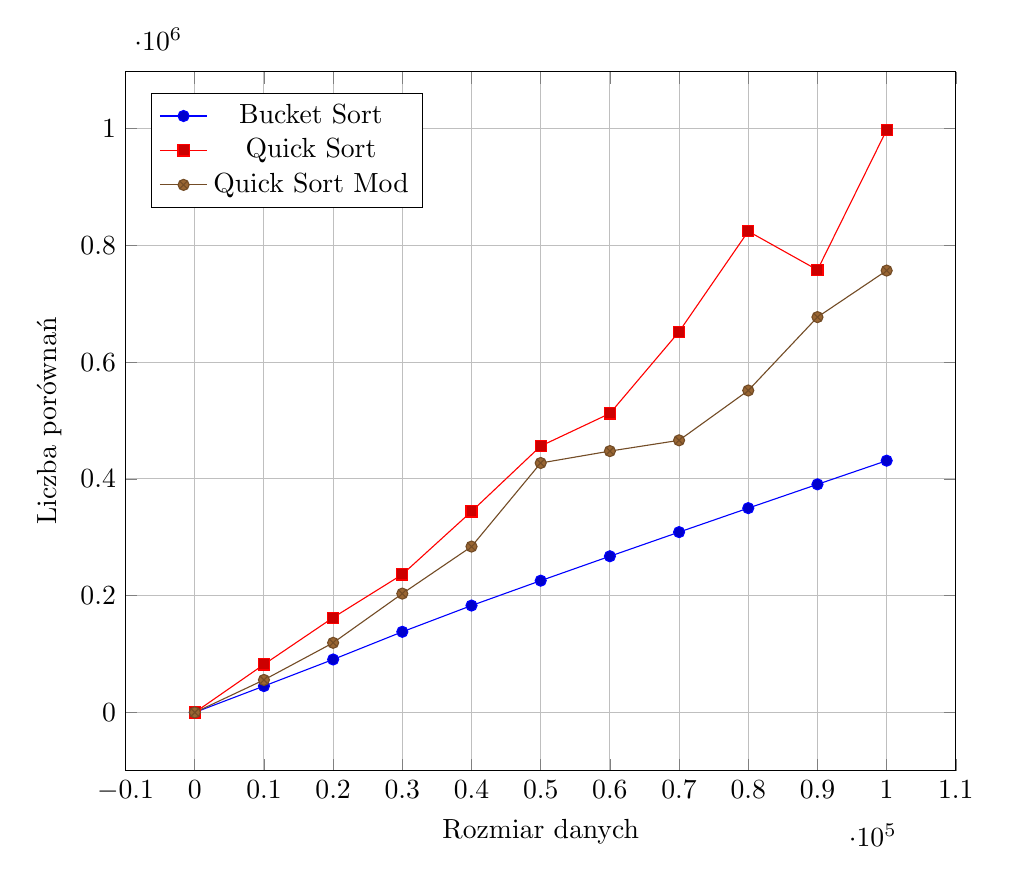
\begin{tikzpicture}
        \begin{axis}[
            width=\textwidth,
            xlabel={Rozmiar danych},
            ylabel={Liczba porównań},
            legend pos=north west,
            grid=major,
        ]
        
        \addplot coordinates {(10, 43 ) (10000, 45139 ) (20000, 90700 )  (30000, 138077 )  (40000, 183047 )  (50000, 225665 )  (60000, 267487 )  (70000, 308844 )  (80000, 349898 )  (90000, 390646 ) (100000, 431179 )};
        \addplot coordinates {(10, 21 ) (10000, 82193 ) (20000, 162436 )  (30000, 236312 )  (40000, 344173 )  (50000, 456204 )  (60000, 512061 )  (70000, 652057 )  (80000, 824061 )  (90000, 757839 ) (100000, 997581 )};
        \addplot coordinates {(10, 5 ) (10000, 55684 ) (20000, 119223 )  (30000, 203510 )  (40000, 284069 )  (50000, 427192 )  (60000, 447591 )  (70000, 466037 )  (80000, 551391 )  (90000, 677047 ) (100000, 756789 )};
        \legend{Bucket Sort, Quick Sort, Quick Sort Mod}
        \end{axis}
    \end{tikzpicture}
    \caption{Liczba porównań w zależności od rozmiaru danych}
\end{figure}

\begin{figure}[H]
    \centering
    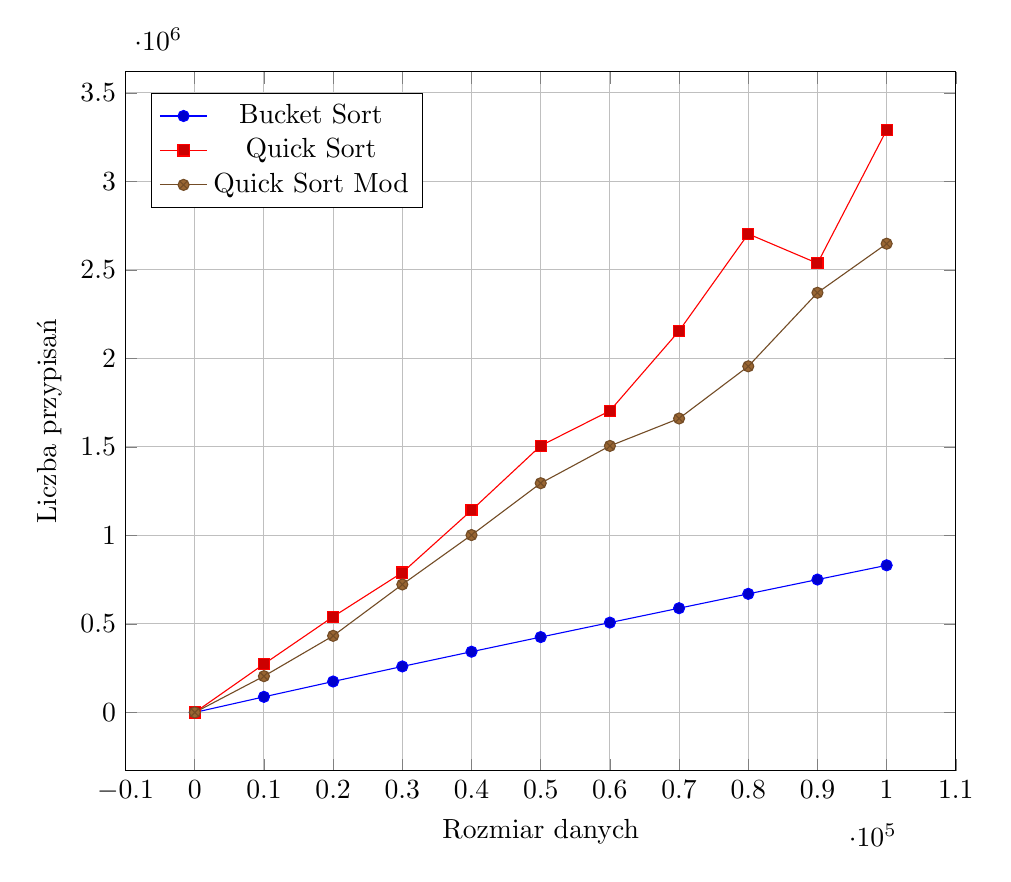
\begin{tikzpicture}
        \begin{axis}[
            width=\textwidth,
            xlabel={Rozmiar danych},
            ylabel={Liczba przypisań},
            legend pos=north west,
            grid=major,
        ]
        
        \addplot coordinates {(10, 94 ) (10000, 88055 ) (20000, 174766 )  (30000, 259789 )  (40000, 343068 )  (50000, 425680 )  (60000, 507504 )  (70000, 588861 )  (80000, 669919 )  (90000, 750668 ) (100000, 831200 )};
        \addplot coordinates {(10, 91 ) (10000, 273283 )  (20000, 540888 )  (30000, 790156 )  (40000, 1141947 )  (50000, 1506584 )  (60000, 1703999 )  (70000, 2155167 )  (80000, 2703351 )  (90000, 2537233 )  (100000, 3290535 )};
        \addplot coordinates {(10, 50 ) (10000, 204785 ) (20000, 432713 )  (30000, 722921 )  (40000, 1002039 )  (50000, 1295001 )  (60000, 1505595 )  (70000, 1660616 )  (80000, 1955348 )  (90000, 2370927 ) (100000, 2648037 )};
        \legend{Bucket Sort, Quick Sort, Quick Sort Mod}
        \end{axis}
    \end{tikzpicture}
    \caption{Liczba przypisań w zależności od rozmiaru danych}
\end{figure}

\begin{figure}[H]
    \centering
    \begin{tikzpicture}
        \begin{axis}[
            width=\textwidth,
            xlabel={Rozmiar danych},
            ylabel={Czas (\mu s)},
            legend pos=north west,
            grid=major,
        ]
        
        \addplot coordinates {(10, 4 ) (10000, 1312 )  (20000, 2734 )  (30000, 4233 )  (40000, 6234 )  (50000, 9371 )  (60000, 10745 )  (70000, 11899 )  (80000, 13763 )  (90000, 14901 )  (100000, 18424 )};
        \addplot coordinates {(10, 0.12 ) (10000, 1217 )  (20000, 2634 )  (30000, 4139 )  (40000, 5962 )  (50000, 7410 )  (60000, 8829 )  (70000, 10487 )  (80000, 12772 )  (90000, 13202 )  (100000, 16752 )};
        \addplot coordinates {(10, 0.11 ) (10000, 1083 )  (20000, 2290 )  (30000, 3533 )  (40000, 5144 )  (50000, 6540 )  (60000, 8410 )  (70000, 8592 )  (80000, 10213 )  (90000, 11661 )  (100000, 13799 )};
        \legend{Bucket Sort, Quick Sort, Quick Sort Mod}
        \end{axis}
    \end{tikzpicture}
    \caption{Czas wykonania w zależności od rozmiaru danych}
\end{figure}
\newpage
\subsection{Tabela Wyników Radix Sort}
\begin{longtable}{|c|c|c|c|c|c|c|}
\hline
Rozmiar danych & Podstawa & Algorytm & Porównania & Przypisania & Czas(s) \\
\hline
10 & 10 & Radix Sort & 0 & 147 & 2\mu s \\
10 & 10 & Radix Sort Neg & 0 & 160 & 8\mu s \\
10 & 100 & Radix Sort & 0 & 359 & 1\mu s \\
10 & 100 & Radix Sort Neg & 0 & 100 & 4\mu s \\
\hline
1000 & 10 & Radix Sort & 0 & 10057 & 83\mu s \\
1000 & 10 & Radix Sort Neg & 0 & 16000 & 111\mu s \\
1000 & 100 & Radix Sort & 0 & 6309 & 49\mu s \\
1000 & 100 & Radix Sort Neg & 0 & 10000 & 67\mu s \\
\hline
10000 & 10 & Radix Sort & 0 & 100057 & 858\mu s \\
10000 & 10 & Radix Sort Neg & 0 & 160000 & 922\mu s \\
10000 & 100 & Radix Sort & 0 & 60309 & 496\mu s \\
10000 & 100 & Radix Sort Neg & 0 & 100000 & 733\mu s \\
\hline
100000 & 10 & Radix Sort & 0 & 1000056 & 8517\mu s \\
100000 & 10 & Radix Sort Neg & 0 & 1600000 & 9156\mu s \\
100000 & 100 & Radix Sort & 0 & 600308 & 4917\mu s \\
100000 & 100 & Radix Sort Neg & 0 & 1000000 & 5701\mu s \\
\hline
\caption{Porównanie liczby operacji dla różnych rozmiarów danych i baz}
\label{tab:results}
\end{longtable}
\subsection{Wykresy Wyników Radix Sort}
Poniżej przedstawiono wykres przedstawiający jak wygląda czas działania Radix Sort i jego modyfikacji dla tabeli rozmiaru 10000 i różnych baz.
\newpage
\begin{figure}[H]
    \centering
    \begin{tikzpicture}
        \begin{axis}[
            width=\textwidth,
            xlabel={Baza},
            ylabel={Czas (\mu s)},
            legend pos=north west,
            grid=major,
        ]
        
        \addplot coordinates {(10, 829 ) (20, 651 )  (30, 649 )  (40, 501 )  (50, 490 )  (60, 539 )  (70, 547 )  (80, 520 )  (90, 492 )  (100, 491 )};
        \addplot coordinates {(10, 921 ) (20, 743 )  (30, 732 )  (40, 573 )  (50, 611 )  (60, 574 )  (70, 573 )  (80, 570 )  (90, 568 )  (100, 569 )};
        \legend{Radix Sort, Rdaix Sort Neg}
        \end{axis}
    \end{tikzpicture}
    \caption{Czas wykonania w zależności od bazy}
\end{figure}
\newpage
\section{Wnioski}

Przeprowadzone badania pozwalają dostrzec, jak różne algorytmy sortowania zachowują się w zależności od danych i parametrów. W przypadku algorytmu Radix Sort, zmiana bazy (liczby elementów, na które dzielimy dane w każdym przebiegu) ma istotny wpływ na liczbę wymaganych iteracji oraz operacji. Wraz ze wzrostem bazy liczba iteracji maleje, ponieważ więcej bitów liczby jest przetwarzanych jednocześnie. Jednak zwiększenie bazy zwiększa złożoność operacji na pojedynczym przebiegu, co może wpłynąć na ogólną wydajność.

Porównanie Quick Sort z Bucket Sort wykazało, że Quick Sort jest zazwyczaj szybszy w praktyce, szczególnie dla większych zbiorów danych, dzięki swojej efektywności w wykorzystaniu pamięci podręcznej i dobrze zbalansowanym podziałom. Mimo to, Quick Sort wykonuje znacznie więcej operacji w porównaniu z Bucket Sort, co może czynić ten drugi bardziej efektywnym w specyficznych przypadkach, zwłaszcza przy równomiernie rozłożonych danych.

Podsumowując, wybór odpowiedniego algorytmu zależy od charakterystyki danych wejściowych oraz wymagań dotyczących wydajności i złożoności obliczeniowej.

\end{document}
